% !TeX root = ../main.tex
\section{Introduction}
Mixture-of-experts (MoE) models increase parameter capacity through sparse activation~\cite{shazeer,switch,mixtral,deepseekmoe}.
Each token executes a few experts in each layer, but deployment requires access to the entire expert pool.
The stored weights grow with the pool even when the active set stays small.
CPU offloading adds host memory to GPU high-bandwidth memory (HBM), extending the space available for weights.
Expert weights share memory with dense parameters, activations, and the KV cache.
Once expert weights exceed this combined capacity, deployment requires a backing store~\cite{flexgen}.
Offline workloads for LLMs include model evaluation, information extraction, and form processing~\cite{flexgen,lightning}.
On workstations and shared servers, a hard disk drive (HDD) can provide this backing storage.
HBM and CPU memory cache part of the pool, while HDD retains its complete weights.
An HBM resident executes directly.
A CPU resident requires a host-to-device (H2D) copy.
An expert absent from both tiers requires an HDD read followed by H2D.
These paths recur as generation revisits the layers for each output token.
The task manages this hierarchy within its assigned GPU and host memory.
Placement determines which requests use HDD.
Retention determines which fetched experts remain available for reuse.

Offloading combines expert caching~\cite{offloading,swapmoe,moeinfinity,promoe} with CPU/GPU execution~\cite{fiddler,daop,lightning}.
Recent designs use access analysis for initialization and online replacement~\cite{core}, retain host copies~\cite{ssdllama}, and account for storage access in replacement~\cite{flashmoe}.
HDD-backed execution brings these decisions together over the lifetime of a request stream.
Promotion consumes GPU space and releases host space; coordinating these events preserves reusable experts.
The resulting resident set covers requests across both tiers and persists between inputs, connecting startup decisions to later weight reuse.


Three challenges arise along this lifecycle (Figure~\ref{fig:intro}(a)).
\emph{Cold start} requires fetching the first input's experts from HDD when caches begin empty.
\emph{Repeated reads} occur when independently managed tiers retain overlapping entries and lose other reusable experts.
After $t_1$, $b$ occupies both tiers, while $a$ has left both.
Its next use at $t_2$ reads HDD again.
\emph{Dynamic cache adaptation} changes residency as task demand shifts.
At $t_3$, task B requests $e,b,e$.
Admitting $e$ displaces $b$ from CPU before its next use.
Serving the new task then fetches both the newly selected $e$ and the previously loaded $b$.

\begin{figure}[!t]
\centering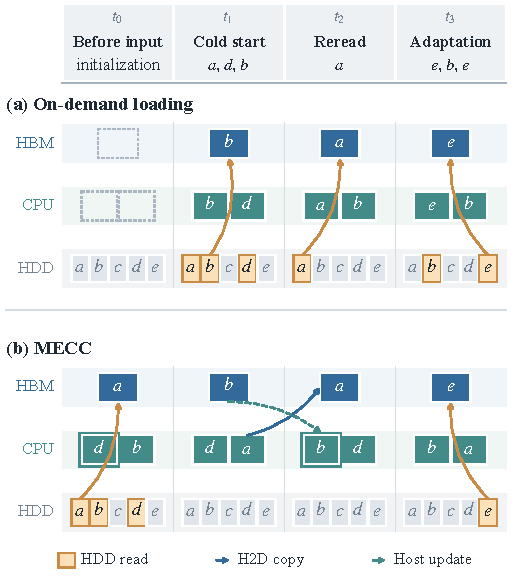
\includegraphics[width=\columnwidth]{figures/fig01_demand_lifecycle.pdf}
\par\nointerlineskip
\caption{On-demand loading (a) and MECC (b) over one request lifecycle.
Each has one HBM slot and two CPU slots.
Orange paths show HDD fetches during each stage; dashed links update host membership.}
\label{fig:intro}
\end{figure}

We present \mecc{} (MoE Expert Cache Coordination), which combines a planned initial placement with request-driven caching.
Figure~\ref{fig:intro}(b) follows the same request lifecycle.
Offline analysis counts expert selections separately for each layer.
The expert planner ranks experts within each layer and allocates HBM/CPU slots by marginal demand coverage.
It compares the next uncovered rank across layers to choose where an added slot covers more demand.
The plan specifies per-layer capacities and the initial expert IDs.
Preloading $a$ into HBM and $d,b$ into CPU memory covers the first input.
When $a$ promotes at $t_2$, the freed CPU slot retains $b$ through a metadata update to its host mirror.
Task B first loads $e$ from HDD.
Subsequent requests to $b,e$ hit CPU after promotion and demotion update the joint recency order.
This replaces the initial membership with experts selected by the new task.
Per-layer capacities stay fixed, and cache state persists across tokens and requests.
Weight delivery completes each required read and H2D copy before the corresponding expert executes.
The router selects the experts, and each executes with its own FP16 weights.
The implementation is available at \url{https://anonymous.4open.science/r/MECC-949C/}.

Our contributions are as follows.
\begin{list}{}{\setlength{\leftmargin}{16pt}\setlength{\labelwidth}{14pt}\setlength{\labelsep}{2pt}\setlength{\itemsep}{9pt}\setlength{\topsep}{6pt}}
\item[(1)] We propose an expert planner for MoE deployment on one GPU.
It allocates HBM/CPU capacity across layers by marginal demand coverage and selects initial expert residents using offline routing analysis.
\item[(2)] We propose a retention mechanism that reuses CPU slots released by promotion.
It links HBM replacement to CPU admission, keeping the displaced expert's host copy available for reuse and saving a device-to-host transfer.
\item[(3)] We propose a request-driven policy that adapts expert residency to changes in task demand.
The policy updates the initial resident set through a joint HBM/CPU recency order, preserving per-layer capacities and cache state across tokens and requests.
\end{list}

